\documentclass[11pt,a4paper]{article}

% Utilisation du style SOBA (défini dans soba.sty)
\usepackage{soba}
%\setlength{\headsep}{50pt}
% ---------------------------
% DÉBUT DU DOCUMENT
% ---------------------------
\begin{document}

% Page de garde
\begin{titlepage}
    \centering
    \vspace*{2cm}
    
    % Logo
    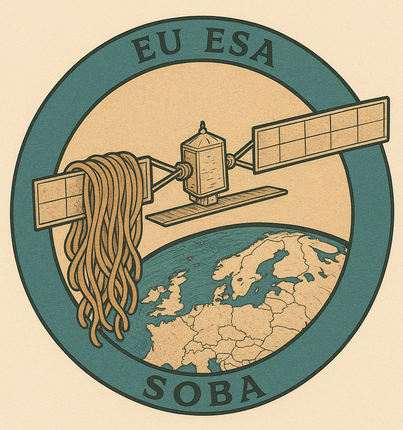
\includegraphics[width=0.4\textwidth]{logo_soba.png}
    
    \vspace{2cm}
    
    {\Huge \textbf{SOBA Project} \par}
    \vspace{1cm}
    {\Large \textbf{Technical documentation for \hl{dataset name} Co-aligned Parquet Catalogue description} \par}
    
    \vspace{2cm}
    
    \textbf{Work Package 3: Datasets Preparation} \\
    \vspace{0.5cm}
    
    \vfill
    
    \begin{center}
    \begin{tabular}{ll}
        \textbf{Authors} & SOBA consortium \\
        \textbf{Intended Audience} & internal \\
        \textbf{Project delivrable document identifier} & TN5 \\
    \end{tabular}
    \end{center}
    
    \vspace{1cm}
\end{titlepage}

\tableofcontents

\newpage

\textbf{Scope:} This document describes one of the co-aligned catalogue parquet datasets produced in the framework of the SOBA project. It details the dataset content, and the way the dataset has been generated.


% Utilisation du diagramme avec légende
\begin{figure}[htbp]
    \centering
    %documentclass[a4paper,landscape]{article}.txt
%\documentclass[a4paper,landscape]{article}
%\usepackage[margin=1cm]{geometry}
%\usepackage{tikz}

\usetikzlibrary{shapes.geometric, arrows, positioning, calc}

%\begin{document}

\pagestyle{empty}

\tikzset{
    input/.style = {rectangle, draw, fill=orange!30, text centered, minimum height=0.7cm, minimum width=2.2cm, rounded corners=2pt, align=center, font=\small\sffamily},
    tool/.style  = {rectangle, draw, fill=blue!30, text centered, minimum height=0.7cm, minimum width=2.2cm, rounded corners=2pt, align=center, font=\small\sffamily},
    dataset/.style = {rectangle, draw, fill=green!30, text centered, minimum height=0.7cm, minimum width=2.2cm, rounded corners=0pt, align=center, font=\small\sffamily},
    highlight/.style = {dataset, draw=red!90!black, thick, font=\small\sffamily\bfseries},  % <-- nouveau style
    arrow/.style = {thick, -stealth},
}

\begin{tikzpicture}[node distance=0.8cm and 1.5cm]

% ---- Entrées ----
\node[input] (A) {S-1 ESA products};
\node[input, below=0.8cm of A] (B) {APIs: CDSE, \\ EODMSRapids, \\ PODAAC SWOT};
\node[input, below=0.8cm of B] (C) {reference products\\ at Ifremer};

% ---- Outil de construction des matchups ----
\node[tool, right=1.5cm of A] (build_match) {tool to \\ build matchups};

\draw[arrow] (A) -- (build_match);
\draw[arrow] (B) -- (build_match);
\draw[arrow] (C) -- (build_match);
% ---- Dataset matchups ----
\node[dataset, right=1.8cm of build_match] (matchups) {matchups files};

\draw[arrow] (build_match) -- (matchups);

% ---- Branche 1 : co-aligned -> split -> test (à gauche) ----
% Départ diagonal vers le bas-gauche (angle 225°)
\node[tool, below left=2.2cm and 1.0cm of matchups] (coalign) {tool to \\ build co-aligned};
\node[highlight, below=0.8cm of coalign] (coaligned_dataset) {co-aligned parquet};  % <-- style highlight
\node[tool, below=0.8cm of coaligned_dataset] (split) {tool to \\ split co-aligned};
\node[dataset, below=0.8cm of split] (splitout) {splited listings};
\node[tool, below=0.8cm of splitout] (gentest) {tool to \\ build test};
\node[dataset, below=0.8cm of gentest] (test) {test dataset};

\draw[arrow] (matchups.south) -- (coalign.north); % diagonale directe

\draw[arrow] (coalign) -- (coaligned_dataset);
\draw[arrow] (coaligned_dataset) -- (split);
\draw[arrow] (split) -- (splitout);
\draw[arrow] (splitout) -- (gentest);
\draw[arrow] (gentest) -- (test);

% ---- Branche 2 : co-locations -> training -> train & val (à droite) ----
% Départ diagonal vers le bas-droit (angle 315°)
\node[tool, below right=2.2cm and 1.0cm of matchups] (coloc_builder) {tool to \\ build co-locations};
\node[dataset, below=0.8cm of coloc_builder] (coloc) {co-locations};
\node[tool, below=0.8cm of coloc] (train_builder) {tool to \\ build training};
\node[dataset, below left=0.6cm and 0.5cm of train_builder] (train) {train dataset};
\node[dataset, below right=0.6cm and 0.5cm of train_builder] (val) {val dataset};

\draw[arrow] (matchups.south) -- (coloc_builder.north);

\draw[arrow] (coloc_builder) -- (coloc);
\draw[arrow] (coloc) -- (train_builder);
\draw[arrow] (train_builder) -| (train);
\draw[arrow] (train_builder) -| (val);

% ---- Jonction entre les branches : lien de splitout vers coloc_builder ----
\draw[arrow] (splitout) -- (coloc_builder);

\end{tikzpicture}

%\end{document}
    \caption{SOBA Dataflow schema}
    \label{fig:dataflow}
\end{figure}
% Définition du concept (fichier externe cpcd_definition.tex)
% cpcd_definition.tex

\begin{tcolorbox}[colback=lightgray, colframe=esa_teal, title=\textbf{Definition: Coaligned Parquet Catalogue Datasets (CPCD)}]
\textbf{Coaligned Parquet Catalogue Datasets (CPCD)} are intermediate tabulated files that aim to feed both \textbf{training} and \textbf{test} tasks of the SOBA project. 

They contain:
\begin{itemize}
    \item \textbf{Identifier information} (e.g., paths and measurement names associated to a reference dataset),
    \item \textbf{SAR meta-information} (incidence angle, heading angle, polarization, etc.),
    \item \textbf{Ancillary information} such as wind speed/direction (NWP), wave Hs (WW3), rain rate (IMERG), ice (SWOT), and SAR surface roughness texture classification (TenGeoP) to allow tailored datasets.
\end{itemize}

These CPCD are built from co-locations between a reference dataset and a Sentinel-1 SAR image (or piece of image). They are \textbf{agnostic on the SAR subsetting} and on the \textbf{SAR observables} targeted for training downstream tasks. These files are intended as starting points for further data pre-processing.
\end{tcolorbox}

\section*{Version History}
\addcontentsline{toc}{section}{Version History}

\begin{table}[H]
    \centering
    \begin{tabular}{@{}p{2cm}p{3cm}p{8cm}p{4cm}@{}}
        \toprule
        \textbf{Version} & \textbf{Date} & \textbf{Modification} & \textbf{Author} \\
        \midrule
        1.0.0 & 2026-08-29 & Creation of the document & Antoine Grouazel, Ifremer \\
        1.0.1 & 2026-08-30 & Update of the template and figures addition & Antoine Grouazel, Ifremer \\
        1.0.2 & 2026-09-06 & Definition of Catalogue files and version table & Antoine Grouazel, Ifremer \\
        \bottomrule
    \end{tabular}
\end{table}

\newpage

% ---------------------------
% SECTION 1 : Dataset Content Description
% ---------------------------

\section{Dataset Content Description}

\textbf{Dataset general description:} \hl{fill this part with product name, provider, resolution, SAR mode, polarization, unit ...etc}

\subsection{Global Coverage Map}
\textbf{Description:} The co-aligned catalogue offers Sentinel-1 SAR acquisitions (\hl{IW and WV modes}) matched with reference observations. The map below illustrates the spatial distribution of the co-aligned data points (matchups) across the globe.

\begin{figure}[H]
    \centering
    % Placeholder: Remplacez par votre image de carte de couverture globale
    \fbox{\parbox{\textwidth}{\centering \vspace{4cm} \textit{[Insert Global Coverage Map Image Here]} \vspace{4cm}}}
    \caption{Global spatial distribution of the SOBA co-aligned SAR/reference matchups.}
    \label{fig:coverage_map}
\end{figure}

\subsection{Monthly Distribution of Matchups}
\textbf{Description:} To assess the temporal coverage and potential seasonal biases, the number of co-aligned observations per month is plotted below.

\begin{figure}[H]
    \centering
    % Placeholder: Remplacez par votre graphique en barres mensuel
    \fbox{\parbox{0.8\textwidth}{\centering \vspace{3cm} \textit{[Insert Monthly Barchart Image Here]} \vspace{3cm}}}
    \caption{Monthly count of co-aligned SAR/reference matchups in the catalogue.}
    \label{fig:monthly_distribution}
\end{figure}

\subsection{Reference Parameter Distribution}
\textbf{Description:} The statistical distribution of the reference \hl{<geophysical parameters>}  is shown below.

\begin{figure}[H]
    \centering
    % Placeholder: Remplacez par votre histogramme
    \fbox{\parbox{0.8\textwidth}{\centering \vspace{3cm} \textit{[Insert 1D or 2D Histogram of Reference Variables Here]} \vspace{3cm}}}
    \caption{Distribution of reference parameters present in the catalogue.}
    \label{fig:ref_distribution}
\end{figure}

\newpage
% ---------------------------
% SECTION 2 : Dataset Production Steps
% ---------------------------
\section{Dataset Production Steps}

\subsection{Selected Products}
The co-aligned catalogue is built from Sentinel-1 SAR products and external reference datasets. 

\begin{itemize}
    \item \textbf{input colocation dataset:} \hl{path or DOI or dataset name}
    \item \textbf{SAR acquisition Mode :} \hl{WV, IW , EW} 
    \item \textbf{Polarizations:} \hl{VV, VH, HH, HV }
\end{itemize}

\textbf{Reference Products:}
\begin{itemize}
    \item Examples: \hl{KNMI-SCAT-HY2B-25km (scatterometer wind), altimetry-derived wave heights, or model reanalysis data (e.g., ERA5).}
    \item The reference product is selected based on its temporal proximity and spatial representativity to the SAR acquisition.
\end{itemize}

\subsection{Selection of Tiles / Filtered Co-locations}
The raw SAR products are processed to extract co-aligned tiles or imagettes that correspond to the reference data points. 
\begin{enumerate}
\item \textbf{geographic delta co-location criteria:}  \hl{to be filled}
\item \textbf{time delta co-location criteria:}  \hl{to be filled}
\end{enumerate}

\textbf{Processing Steps:}
\begin{enumerate}
    \item \textbf{step 1:} \hl{to be filled}
    \item \textbf{step 2:} \hl{to be filled}
    \item ...
\end{enumerate}

\subsection{Libraries and Commands Used}
The catalogue generation pipeline relies on open-source \hl{github/gitlab link} libraries and specific command-line tools. Below is an example of command used for data generation:

\begin{lstlisting}[caption={Example of bash cmd for data generation.}, label={lst:code}]
example of command used.
\end{lstlisting}

\subsection{Configuration Files}
The production pipeline uses YAML/JSON configuration files to define paths, filtering thresholds, and product selection. An example structure is provided below:

\begin{lstlisting}[caption={Example of configuration file \hl{to be modified}  (config.yaml).}, label={lst:config}]
# SOBA Configuration
sar_products:
  mode: "IW"        # Options: IW, WV, EW
  levels: ["L1_GRD", "L1_SLC", "L2_OCN"]
  polarizations: ["VV", "VH"]

reference_products:
  - name: "KNMI-SCAT-HY2B-25km"
    type: "scatterometer"
    variables: ["windspeed_scat", "winddirection_scat"]
    
filters:
  max_time_diff_minutes: 30
  min_distance_to_coast_km: 2.0
  max_incidence_angle_deg: 45.0
\end{lstlisting}

\newpage
% ---------------------------
% BIBLIOGRAPHIE
% ---------------------------
\newpage
\section*{References}
\addcontentsline{toc}{section}{References}

\begin{thebibliography}{9}

\bibitem{soba_format}
SOBA Consortium.
\textit{Format Description for parquet co-aligned datasets}.
Technical Document, Ifremer / Galeio, 2026.
Available at: \url{https://docs.google.com/document/d/1h4bLs1Z67MLL5ws3ckL2zrdYkajXCRGQKpSfnLGABes/edit?usp=sharing}

\end{thebibliography}

\end{document}